\chapter{Общие положения}

\hspace*{1.25cm}Данная глава посвящена формальной постановке задачи предиктивного анализа задержек в конвейере видеоаналитики и представлению архитектуры исследуемой системы. В рамках главы вводятся ключевые математические обозначения, определяются целевые метрики и ограничения, формулируются требования к разрабатываемому алгоритму. Особое внимание уделяется описанию структуры видеоконвейера и точек сбора телеметрических данных, которые лягут в основу построения прогностической модели.

\section{Архитектура системы видеоаналитики}

\hspace*{1.25cm}Исследуемая система видеоаналитики представляет собой многокомпонентный конвейер, предназначенный для обработки видеопотоков в режиме реального времени с применением алгоритмов компьютерного зрения для детекции событий и объектов. Архитектура системы строится по принципу микросервисной архитектуры, что обеспечивает масштабируемость и отказоустойчивость, но одновременно усложняет задачи мониторинга и диагностики производительности.

\hspace*{1.25cm}Видеоконвейер включает следующие основные компоненты: модуль захвата видеопотока с IP-камер (получающий данные по протоколу RTSP), ML-pipeline для применения алгоритмов компьютерного зрения, брокер сообщений Apache Kafka [4] для асинхронной передачи результатов обработки, бэкенд-сервисы для бизнес-логики и сохранения данных, а также WebSocket-клиенты для доставки уведомлений конечным пользователям. Каждый компонент генерирует множество метрик производительности, которые собираются централизованной системой мониторинга Prometheus [2].

\hspace*{1.25cm}Критической характеристикой системы является end-to-end-задержка, измеряемая как время от момента возникновения события в видеопотоке до его отображения на интерфейсе оператора. Данная метрика, обозначаемая как $common\_event\_delay$, напрямую влияет на эффективность работы операторов и качество принимаемых ими решений в критических ситуациях.

\section{Постановка задачи}

\hspace*{1.25cm}Для формальной постановки задачи прогнозирования введем необходимые математические обозначения и определения. Пусть $T=\{t_1, t_2, \ldots, t_n\}$ --- упорядоченное множество временных меток наблюдений, соответствующих моментам сбора метрик из системы мониторинга с фиксированным интервалом дискретизации. Обозначим через $d$ общее число различных метрик, одновременно собираемых системой мониторинга со всех компонентов видеоконвейера.

\hspace*{1.25cm}Для каждой временной метки $t_i$ формируется $d$-мерный вектор наблюдений:

\begin{equation}
	\mathbf{x}_i = [m^{(1)}_i, m^{(2)}_i, \ldots, m^{(d)}_i] \in \mathbb{R}^d,
\end{equation}

где каждая компонента $m^{(j)}_i$ представляет значение $j$-й метрики в момент времени $t_i$.

\hspace*{1.25cm}Компоненты вектора наблюдений соответствуют различным категориям метрик, характеризующих работу отдельных подсистем видеоконвейера:

\begin{itemize}
	\item \textbf{Метрики ML-конвейера:} $vidcap\_delay$ (задержка видеозахвата), $vidcap\_fps$ (частота кадров видеозахвата), $vidcap\_fps\_avg$ (средняя частота кадров видеозахвата), характеризующие производительность модулей компьютерного зрения;
	\item \textbf{Метрики бэкенда:} $ml\_to\_backend\_kafka\_delay$ (задержка передачи результатов ML через Kafka), $db\_insert\_delay$ (время записи в базу данных), отражающие эффективность серверной части системы;
	\item \textbf{Метрики WebSocket-клиента:} $common\_event\_delay$ (целевая end-to-end-задержка), $heartbeat\_*$ (метрики жизнеспособности соединений), $event\_counter$ (счетчики событий), $seq\_events\_health$ (показатели корректности последовательности событий), характеризующие качество доставки результатов до конечных пользователей.
\end{itemize}

\hspace*{1.25cm}Для учета временных зависимостей в данных введем понятие скользящего окна наблюдений. Определим окно длины $L$ и шаг сдвига $s$, где $L$ представляет глубину истории, необходимую для прогнозирования, а $s$ --- частоту обновления прогнозов. Каждое $k$-е скользящее окно определяется как матрица:

\begin{equation}
	X_k = [\mathbf{x}_{t_k - L + 1}, \ldots, \mathbf{x}_{t_k}] \in \mathbb{R}^{L \times d},
\end{equation}

содержащая $L$ последовательных векторов наблюдений, предшествующих моменту прогнозирования. На основе данной матрицы формируется расширенное множество признаков для обучения модели, включающее различные статистические агрегаты, временные лаги и производные характеристики, детальное описание которых приводится в главе 2.

\hspace*{1.25cm}Целевая переменная для задачи прогнозирования определяется как значение критической метрики end-to-end-задержки в будущий момент времени:

\begin{equation}
	y_k = common\_event\_delay(t_k + \Delta),
\end{equation}

где $\Delta = 900 \times 15$ с $= 13500$ с $\approx 3{,}75$ ч представляет горизонт прогнозирования, выбранный исходя из требований к заблаговременности предупреждений о потенциальных проблемах в системе. Данный горизонт соответствует прогнозу на 900 временных шагов вперед при интервале дискретизации 15 секунд.

\hspace*{1.25cm}Обучающая выборка для построения прогностической модели формируется как множество пар «окно-целевое значение»:

\begin{equation}
	\mathcal{N} = \{(X_k, y_k)\}_{k=1}^{N},
\end{equation}

где $N$ --- общее количество доступных обучающих примеров, определяемое длиной исторических данных и параметрами скользящего окна.

\hspace*{1.25cm}В рамках данной постановки предполагается существование неизвестной целевой функции:

\begin{equation}
	f^*: \mathbb{R}^{L \times d} \to \mathbb{R},
\end{equation}

которая отображает текущее состояние системы (представленное матрицей метрик скользящего окна) в прогнозируемое значение end-to-end-задержки. 

\hspace*{1.25cm}Основная задача исследования состоит в построении алгоритма $A: \mathbb{R}^{L \times d} \to \mathbb{R}$, аппроксимирующего неизвестную функцию $f^*$ с заданной точностью:

\begin{equation}
	|A(X_k) - f^*(X_k)| \le \varepsilon \quad \forall k,
\end{equation}

где $\varepsilon$ --- допустимая погрешность прогнозирования, определяемая практическими требованиями к системе предупреждения.

\hspace*{1.25cm}К разрабатываемому алгоритму $A$ предъявляется ряд требований:

\begin{enumerate}
	\item \textbf{Точность прогнозирования:} обеспечение качества прогноза целевой метрики $common\_event\_delay$ с MAPE $< 10\%$ и других метрик (MAE, RMSE) на валидационной выборке;
	\item \textbf{Производительность:} время формирования прогноза $< 5$ с при развертывании в контейнеризованной среде [5] для практического применения в системе мониторинга;
	\item \textbf{Интерпретируемость:} возможность анализа важности признаков и понимания логики принятия решений моделью;
	\item \textbf{Практичность:} простота интеграции в существующую инфраструктуру мониторинга и возможность автоматизации процесса обновления модели.
\end{enumerate}

\hspace*{1.25cm}Исходные данные для обучения и валидации алгоритма представляют собой многомерный временной ряд $X \in \mathbb{R}^{n \times d}$ с элементами типа FLOAT64, формируемый из системы мониторинга Prometheus с периодичностью сбора 15 секунд. Объем доступных исторических данных составляет приблизительно 90643 точки, накопленные за период 16 дней непрерывной работы системы.

\hspace*{1.25cm}Итоговая формализация задачи: построить алгоритм $A$, наилучшим образом аппроксимирующий неизвестную функцию $f^*$ и одновременно удовлетворяющий всем указанным ограничениям по точности, производительности и адаптивности для обеспечения надежного предиктивного мониторинга систем видеоаналитики.

\begin{landscape}
\vspace*{\fill}
\begin{figure}[H]
	\centering
	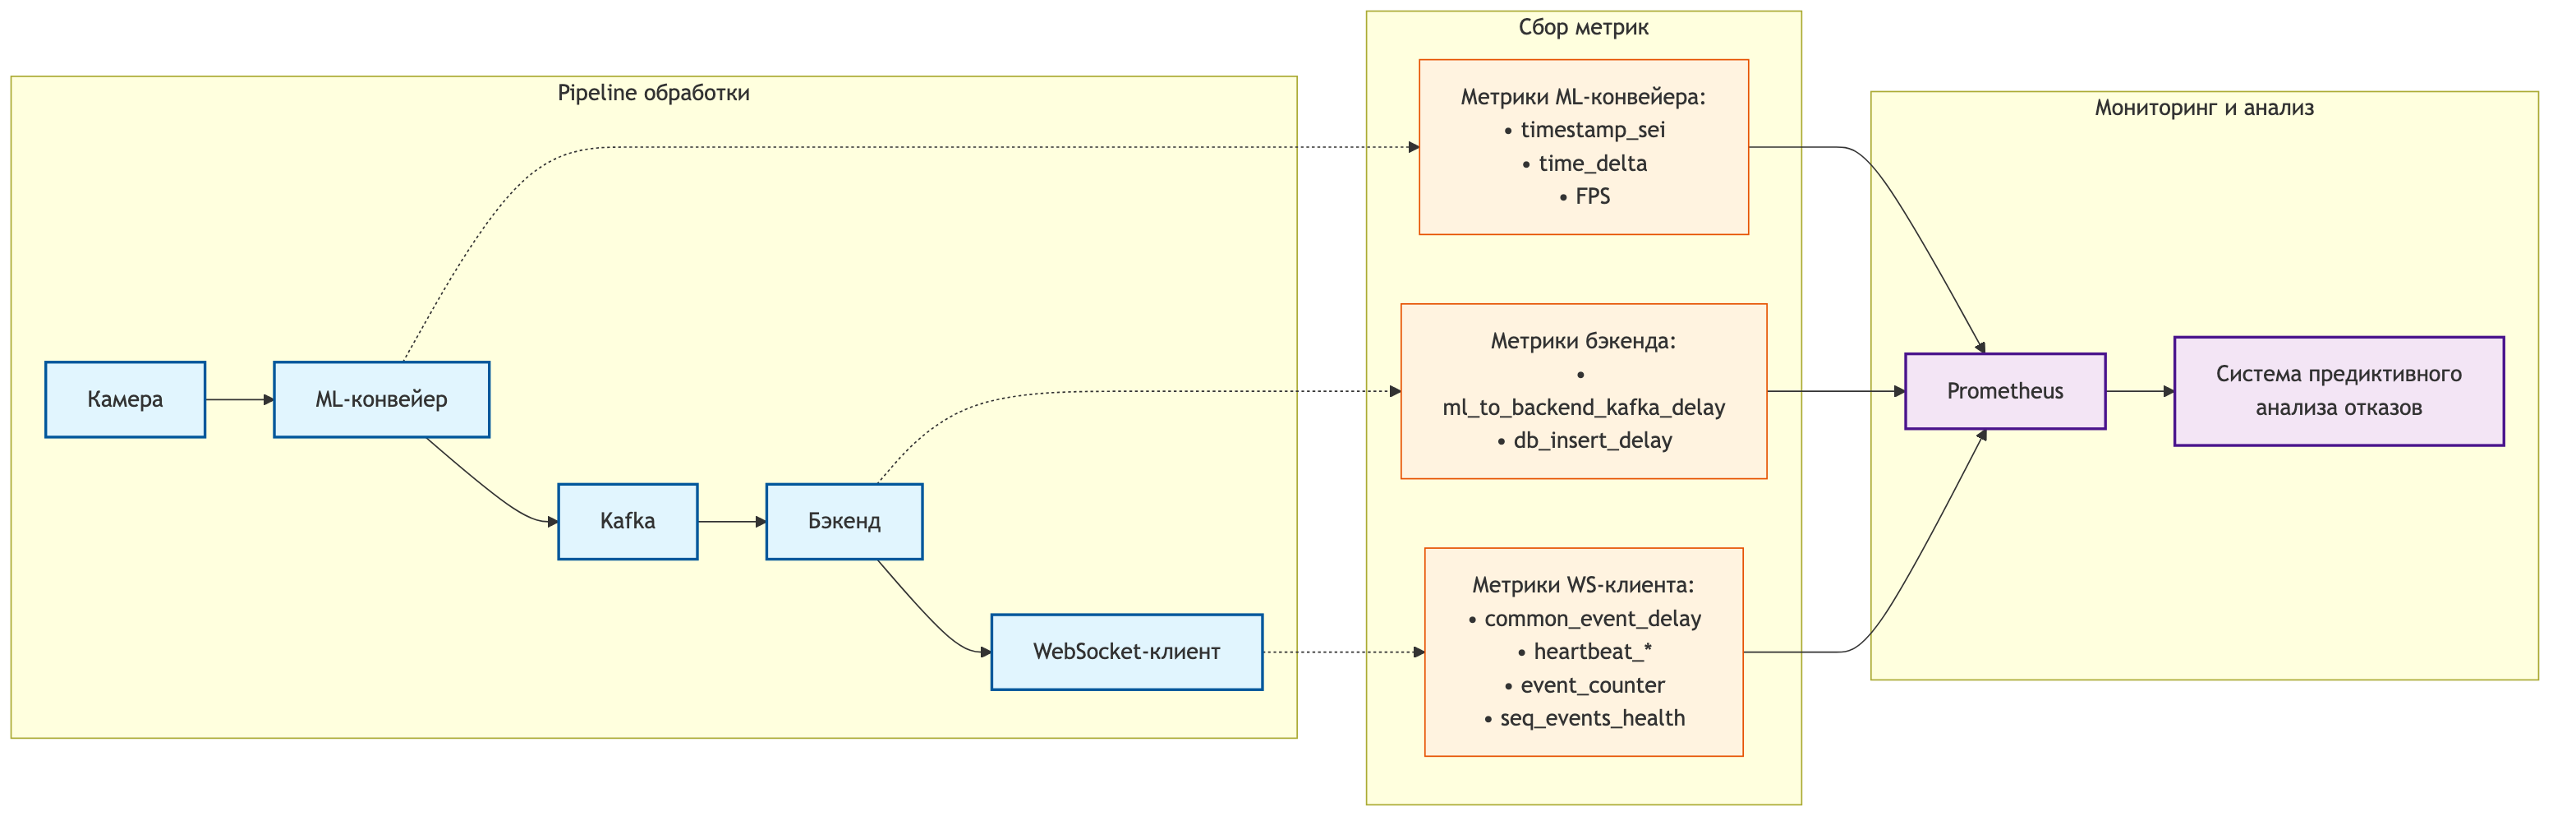
\includegraphics[width=\linewidth,height=\textheight,keepaspectratio]{figures/chapter1/video_pipeline_diagram.png}
	\caption*{Рисунок~1.1 --- Схема видеоконвейера и точки сбора метрик}
	\label{fig:video_pipeline}
\end{figure}
\vspace*{\fill}
\end{landscape}
